\beginpgfgraphicnamed{fig_symm_mps}
\tikzset{gamma/.style={circle=2pt,draw=black!100,fill=blue!20,inner sep=3pt}}
\tikzset{spin/.style={circle=1pt,draw=black!100,fill=orange!80,inner sep=2pt}}

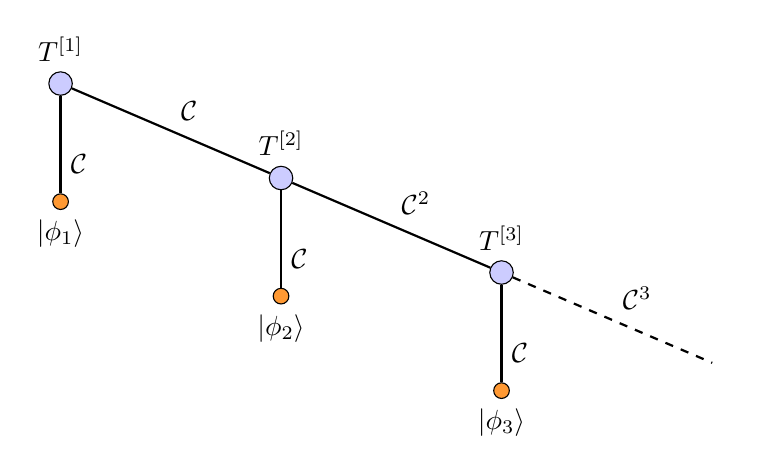
\begin{tikzpicture}[auto]

\foreach \i / \j in {1/0,2/1,3/2}
{
	\node (G\i) at (2.8*\j,-1.2*\j) [gamma] {};
	\node (S\i) at (2.8*\j,-1.5-1.2*\j) [spin] {};
	
	\node[above] (Gl\i) at (G\i.north) {$T^{[\i]}$};
	\node[below] at (S\i.south) {$| \phi_{\i} \rangle$};
	\draw[thick] (G\i) -- node[below right] {$\mathcal{C}$} (S\i);
	
	% \ifnum \j > 0
	% 	\draw[thick] (G\i) -- node[above right] {$c=\lbrace +,- \rbrace$} (G\j);
	% \fi
}

\draw[thick] (G1) -- node[above right] {$\mathcal{C}$} (G2);
\draw[thick] (G2) -- node[above right] {$\mathcal{C}^2$} (G3);

\node (out) at (2.8*3,-3*1.2) {};
\draw[thick,dashed] (G3) -- node [above right] {$\mathcal{C}^3$}(out);

\end{tikzpicture}
\endpgfgraphicnamed